\chapter{光沿直线传播}\label{ch:g4:light-straight-lines}

阳光斜穿过树林间的清晨薄雾 ---
一道道笔直如拉紧的细绳。积满灰尘的阁楼里，手电筒
射出一道边缘锐利的光束。你能听见朋友
在拐角外呼唤你，却无法\emph{看见}他们。
这些现象都是同一条定律的不同表现——
光学中最古老的定律。

\section{直线传播定律}

\begin{proposition}[光沿直线传播]\label{prop:g4:light-straight-lines:law}
在空气中（水、玻璃或真空中同样如此），光沿直线传播。
光不会绕过拐角弯曲，也不会像烟雾那样飘移，
不会为了找到你而绕过墙壁。
若光源发出的直线无法到达某处，
则该处便接收不到来自此光源的光。
\end{proposition}

\begin{definition}[光线]\label{def:g4:light-straight-lines:ray}
为了画出光，物理学家使用\emph{光线}\index{光线}：
一条带箭头的直线，表示一缕光的传播路径。
手电筒的光束可画成一束扇形的光线；
细激光束则只画一条光线。与力的箭头相似，光线是一幅小小的图示，
其中蕴含着一条定律：光的路径，
笔直得如同用尺画出。
\end{definition}

\begin{omfigure}
\begin{tikzpicture}[scale=0.85]
  \draw[thick, fill=omExo, fill opacity=0.3]
    (0.2,1.3) rectangle (1.4,2.3);
  \draw[thick] (1.4,1.45) -- (1.4,2.15);
  \draw[-Stealth, omThm, thick] (1.4,2.1) -- (10.6,2.9);
  \draw[-Stealth, omThm, thick] (1.4,1.8) -- (10.6,1.8);
  \draw[-Stealth, omThm, thick] (1.4,1.5) -- (10.6,0.7);
  \node[below, font=\small] at (0.8,1.1) {手电筒};
  \node[above, font=\small] at (6.0,2.75)
    {扇形光线：条条笔直};
\end{tikzpicture}

{\small 物理学家画法下的手电筒光束：笔直的光线，
箭头标明光的传播方向。}
\end{omfigure}

\begin{example}[定律的表现]\label{ex:g4:light-straight-lines:sightings}
知道了这条定律，你便会处处看见它：穿过薄雾或百叶窗的笔直阳光；
尘埃飞扬的空气中，手电筒光束锐利笔直的边缘；
激光笔那笔直的细线；以及每一座灯塔
扫过夜海的笔直光束。
光线弯曲从未被看见——喷泉和森林可以弯，
光却不会。
\end{example}

\begin{omfigure}
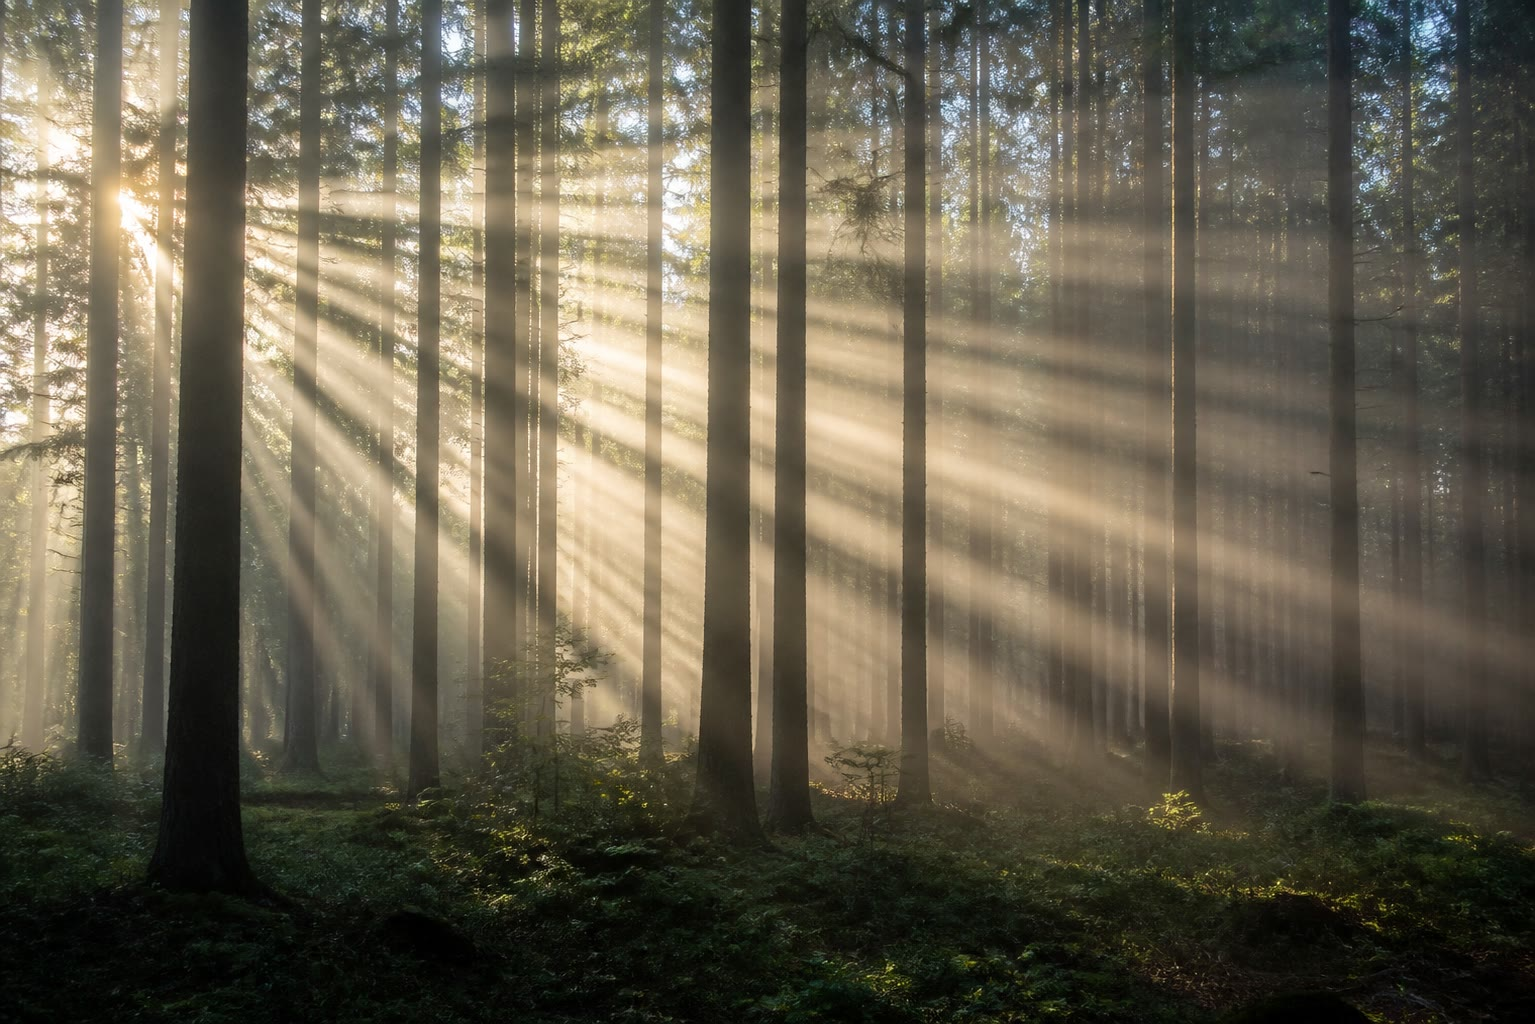
\includegraphics[width=0.58\linewidth]{images/book1/ai/g4-light-sunbeams.jpg}

{\small 大自然的证明：穿过薄雾的阳光笔直无比——光并不会绕过树木弯曲。}
\end{omfigure}

\section{用三张卡片证明}

\begin{method}[三卡实验]\label{met:g4:light-straight-lines:cards}
\begin{enumerate}
  \item 在三张硬卡片的正中央打一个小孔，
        孔的高度须相同；
  \item 将卡片竖直排成一行，相距一掌宽，并在最后一张卡片之后
        放一支点燃的蜡烛（或手电筒）；
  \item 移动头部，直到透过三个小孔看见火焰——
        只有当三个小孔与火焰位于同一条直线上时才能做到
        （检验方法：用一根拉紧的细线穿过小孔，
        看它能否到达火焰）；
  \item 现在将中间那张卡片向旁边平移一指宽。
\end{enumerate}
火焰随即消失。光本可以折线传播——穿过第一个孔，
侧向移动一下，穿过移位后的小孔，再到达你的眼睛——
但它并不这样走：没有直线，就没有光。
\end{method}

\begin{omfigure}
\begin{tikzpicture}[scale=0.85]
  \draw[thick] (1.0,0.3) -- (1.0,2.5) (3.6,0.3) -- (3.6,2.5)
    (6.2,0.3) -- (6.2,2.5);
  \fill[white] (0.92,1.32) rectangle (1.08,1.48);
  \draw[thick] (0.92,1.32) rectangle (1.08,1.48);
  \fill[white] (3.52,1.32) rectangle (3.68,1.48);
  \draw[thick] (3.52,1.32) rectangle (3.68,1.48);
  \fill[white] (6.12,1.32) rectangle (6.28,1.48);
  \draw[thick] (6.12,1.32) rectangle (6.28,1.48);
  % a real candle: wax body, wick, teardrop flame
  \draw[thick, fill=yellow!15] (8.42,0.3) rectangle (8.78,1.02);
  \draw[thick] (8.6,1.02) -- (8.6,1.16);
  \draw[thick, orange!80!red, fill=yellow!80]
    (8.6,1.16) .. controls (8.44,1.3) and (8.47,1.47) .. (8.6,1.58)
    .. controls (8.73,1.47) and (8.76,1.3) .. (8.6,1.16);
  \fill[orange!90] (8.6,1.27) ellipse (0.045 and 0.08);
  % the ray of light, dead straight through the three holes
  \draw[-Stealth, line width=1.3pt, yellow!75!orange]
    (8.44,1.4) -- (-0.4,1.4);
  \node[below, font=\small] at (8.6,0.05) {蜡烛};
  \node[below, font=\small] at (-0.2,1.2) {眼睛};
  \node[above, font=\small] at (4.6,2.55)
    {三孔共线：看见火焰};
\end{tikzpicture}

{\small 三卡实验：火焰、小孔与眼睛
恰好成一直线时，火焰才可见。移动任一张卡片，
视线便随之消失。}
\end{omfigure}

\begin{example}[影子的成因终于讲清]\label{ex:g4:light-straight-lines:shadows}
现在，你一年级时见过的影子，
终于要揭开它的秘密。光从灯发出，沿直线传播；
小球挡住撞上它的光线；
恰好擦过边缘的光线仍沿直线前行。小球身后，正是直线光线无法到达的地方 ---
影子，其锐利的边缘由最后擦过的光线描画而成。
光线笔直，影子才清晰；
若光线弯曲，每个影子都会变成一团模糊的雾。
\end{example}

\section{看见就是接收光}

\begin{proposition}[看见是怎样发生的]\label{prop:g4:light-straight-lines:seeing}
当物体发出的光沿直线射入你的眼睛时，
你便看见了它 --- 若它是光源，光来自它自身；否则，光来自反射的阳光或灯光。
眼睛并不向外伸出什么去抓取世界：
看见是\emph{接收}，像网接住球一样接住光线。
\end{proposition}

\begin{example}[绕过墙角]\label{ex:g4:light-straight-lines:corner}
你的朋友在校舍的拐角处喊你：你能听见，
却看不见他。声音像池塘里的波纹一样扩散，
绕过墙角的边缘；光则坚持沿笔直的路走，
穿过砖墙，没有任何直线能连接朋友的脸与你的眼睛。
要看见拐角后面的东西，你必须\emph{让光路转弯} ---
给光线一个坚硬、光亮的表面，让它反射。这一招
叫作镜子，它将是下一学年第一章“光”的主角。
\end{example}

\begin{remark}[最快的跑者]\label{rem:g4:light-straight-lines:speed}
我们测得，声音每秒慢跑 \qty{340}{m}。
而光沿着笔直的路径，却是另一个量级：它横穿整个天空，
快到任何计数都跟不上 --- 这就是为什么闪光“立刻”到达，
而雷声却要拖上好几秒才慢吞吞地赶来。究竟有多快？
这个数字大得出奇，我们留到
以后的学年再讲 --- 连同人们为测出它而想出的种种巧妙办法
的故事。
\end{remark}

\section{练习}

\begin{exercise}[$\star$]\label{exo:g4:light-straight-lines:1}
说出本章的定律，并举出两个在户外观察到它的实例。
\end{exercise}

\begin{exercise}[$\star$]\label{exo:g4:light-straight-lines:2}
什么是光线？它的画图表示了哪两件事？
\end{exercise}

\begin{exercise}[$\star$]\label{exo:g4:light-straight-lines:3}
在三卡实验中，究竟在什么时候才能看见火焰？
只做哪一个动作就能让火焰消失？为什么？
\end{exercise}

\begin{exercise}[$\star$]\label{exo:g4:light-straight-lines:4}
光沿直线传播的规律，如何解释影子边缘的锐利？
\end{exercise}

\begin{exercise}[$\star$]\label{exo:g4:light-straight-lines:5}
此刻你正在看这本书。请讲述使这一切成为可能的光，
从灯出发，直到进入你的眼睛。
\end{exercise}

\begin{exercise}[$\star$]\label{exo:g4:light-straight-lines:6}
为什么你能听见拐角处的朋友，却看不见他？
声音与光两位“旅行者” --- 在拐角处各自怎样行动？
\end{exercise}

\begin{exercise}[$\star$]\label{exo:g4:light-straight-lines:7}
钥匙孔、门后亮灯的房间与你的眼睛：在昏暗的走廊里，
你站在何处，才能透过钥匙孔看见灯？请用
一条直线作答。
\end{exercise}

\begin{exercise}[$\star$]\label{exo:g4:light-straight-lines:8}
远处放烟花，爆炸声与闪光，哪个先到？
本学年哪条定律、哪项测量，能解释
这段时间差？
\end{exercise}

\begin{exercise}[$\star$]\label{exo:g4:light-straight-lines:9}
“我看星星时，有东西从眼睛里射出去，去碰它。”
请用
\cref{prop:g4:light-straight-lines:seeing} 纠正这一旧看法 --- 传播的是什么？
朝哪个方向？
\end{exercise}

\begin{exercise}[$\star\star$]\label{exo:g4:light-straight-lines:10}
请画出光线图，设计一种方法，从你的房间内
观察走廊，借用
\cref{ex:g4:light-straight-lines:corner}中提到的镜子技巧：门口的反光面应立在何处，
它又如何改变光线的
路径？（潜艇正是用这一办法，叠加两次，以便看清
波浪之上的景象。）
\end{exercise}

\begin{exercise}[$\star\star$]\label{exo:g4:light-straight-lines:11}
在薄雾的清晨，阳光穿过树林，明显地散成
一道道直线 --- 可你的朋友却说：“我们能看见光束，所以
光一定是悬浮在空中、可以看见的东西。”那么，你们两人
实际看见的究竟是什么？当“光束”出现在雾中或尘埃中时，
在完全洁净的空气中，光束又会是什么样子？
\end{exercise}
